\section{The Hall A High Resolution Spectrometer}

Hall A has two 4 GeV/c High Resolution Spectrometers (HRSs), designated Left (LHRS) and Right (RHRS) corresponding to their orientation when looking downstream along the beam. In order to achieve Hall A's stated goal of $1\%$ absolute cross section accuracy, the HRSs were designed to have $10^{-4}$ particle momentum resolution and $0.1$ mrad in scattering angle resolution. 

Each HRS has four superconducting magnets: three cos$\left(2\theta\right)$ and a racetrack coil dipole. Utilizing a QQDQ magnet setup (named Q1, Q2, D, and Q3), each HRS has a $45\degree$ bending angle in a vertical bending plane. Each HRS has a similar, but unique, detector package that accommodates precise tracking and particle identification (PID). Figure \ref{fig:hrs_mags} shows the magnet layout of the HRSs. The setup is identical on both the Left and Right HRS.

\begin{figure}
\begin{center}
	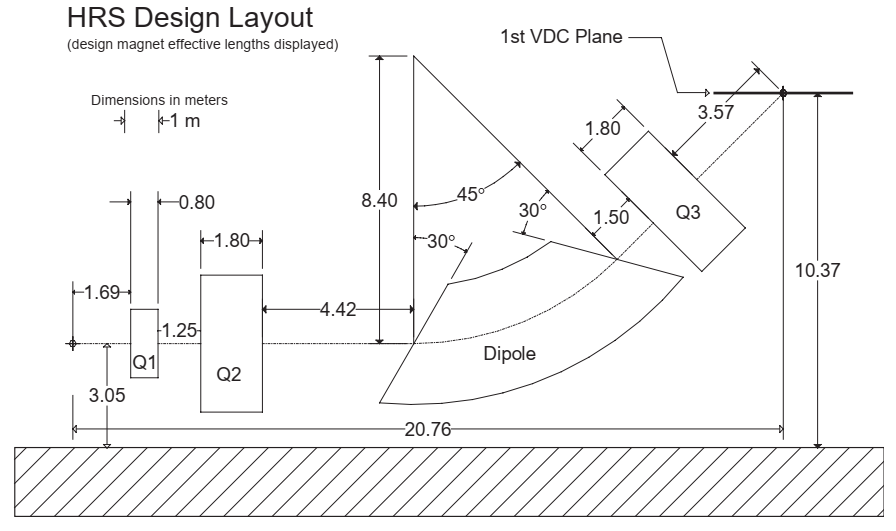
\includegraphics[width=0.8\textwidth]{./setup/fig/HRS_mags.png}
	\caption{A schematic view of the HRS magnet setup. Particles enter from the left in Q1 and then pass through the magnets exiting Q3 into the first VDC plane.\cite{HANIM}}
	\label{fig:hrs_mags}
\end{center}
\end{figure}

The two HRSs can be ran together for exclusive measurements or ran separately for inclusive measurements. MARATHON used each HRS separately in order to maximize counting rate. In particular, the RHRS was parked at the highest angle measurement as the counting rate was very slow.

Each arm consists of a pair of Vertical Drift Chambers (VDCs), two scintillator planes, a gas cherenkov, and two leaded glass calorimeters. This combination of detectors allows for fine tracking and powerful electron identification.

\subsection{Vertical Drift Chambers}

Each arm has two VDCs at the entrance to the detector stack. These detectors are used for fine tracking of particles. Drift chambers are comprised of high voltage planes, sense wires, and a gas mixture. When a particle passes through a drift chamber it ionizes the gas. The high voltage planes keep a constant electric field within the drift chamber. The sense wires are held at ground potential. The ionized gas from incident particles then drifts toward the sense wire creating a build up of charge that can be measured. Using the drift speed of ions in the field and the time that it takes for the ion to reach the sense wire, the position of the track through the VDC can be accurately determined.

The chambers used in the HRSs, as seen in Figure \ref{fig:vdcs}, are oriented parallel to the horizontal plane of the hall and $45\degree$ to the detector stack. The active area of each VDC is 2118 mm by 288 mm. The gas used is an argon (62\%) and ethane(38\%) mixture. The electric field is created by gold-plated Mylar planes spaced 13 mm apart. These planes are held at -4 kV. Each chamber has two wire planes in a UV formation, that is $90\degree$ to each other, that are separated by 335 mm. In each plane there are 368 wires with a wire spacing of 4.24 mm. This setup gives a position resolution of 100 $\mu$m and an angular resolution of 0.5 mrad.

\begin{figure}
\begin{center}
	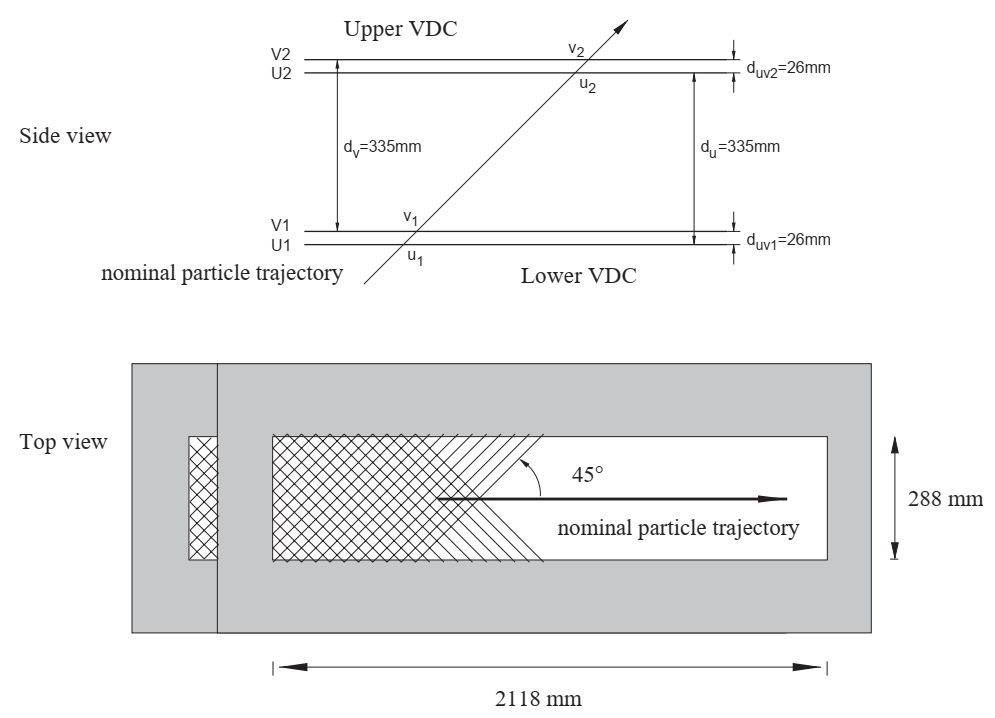
\includegraphics[width=0.8\textwidth]{./setup/fig/vdc.png}
	\caption{A schematic view of the VDCs. These are the first detectors in an HRS.\cite{HANIM}}
	\label{fig:vdcs}
\end{center}
\end{figure}

\subsection{Scintillator Planes}

Each HRS has two scintillator planes that were used for MARATHON: S0 and S2. These two planes sandwich the Gas Cherenkov. The scintillators are plastic paddles with a Photomultiplier Tube (PMT) on each end. When scintillating material is struck by a particle, it absorbs a small amount of energy and emits it as light. The light then travels through the material to the PMTs on each end. When the light reaches the PMT, it knocks electrons out of the photocathode. These electrons are accelerated through a series of exceedingly higher voltage dynodes where more electrons are released. Finally, this cascade reaches the anode with a enough electrons to create a signal that can be read in. This entire process is very quick, allowing the scintillators to be used for setting the timing of events. The time difference between the signal in the PMTs on each end allows for rough tracking.

S0 consists of a single paddle with the PMTs on located on the top and bottom. The S0 paddle made from BICRON 408 scintillating plastic which is 10 mm thick, 170 cm long, and 25 cm wide. The PMTs used are $3''$ XP2312B. There is a trade-off in timing resolution when using a large paddle. The timing resolution of S0 is approximately $0.2ns$.

S2 consists of 16 paddles with the PMTs on the left and right. Each paddle is made from fast plastic scintillator EJ-230 and is 2 inches thick, 17 inches long, and 5.5 inches wide. The paddles are pressed together with a 60 pound force in order to minimize any space between the paddles. The PMTs used are $2''$ Photonis 2282B. Figure \ref{fig:s2} shows the layout of the S2 scintillator plane. In this drawing, particles would pass through the plane of the page. The timing resolution of S2 has been measured to be smaller than $150ps$.

\begin{figure}
\begin{center}
	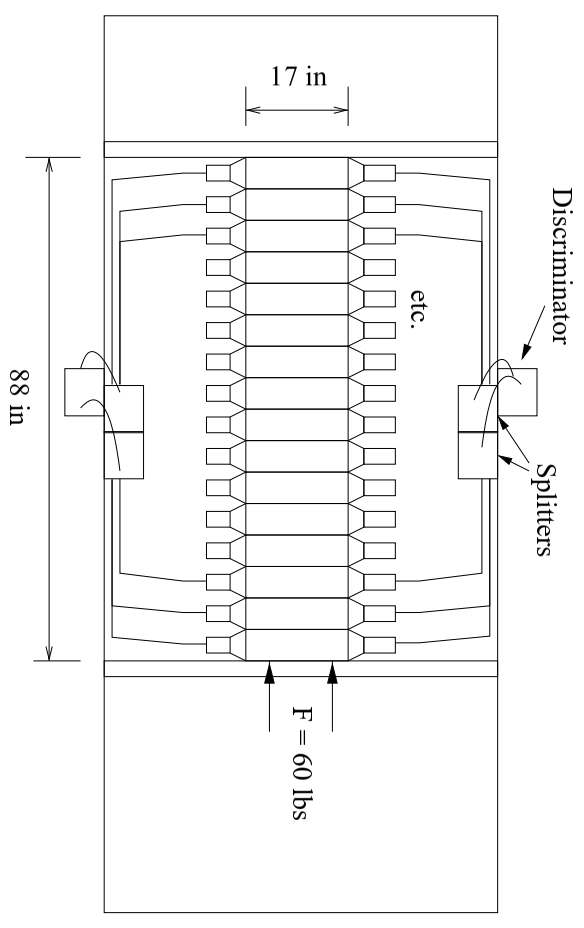
\includegraphics[width=0.3\textwidth]{./setup/fig/s2.png}
	\caption{A schematic drawing of the S2 scintillator plane.\cite{HASEM}}
	\label{fig:s2}
\end{center}
\end{figure}

The signals measured in the scintillators form the basis for the HRS trigger. Since S2 has high time resolution, it serves to set the timing of the event. Proper event timing is critical for the VDCs to accurately track a particle.

\subsection{Gas Cherenkov}
\label{sec:cer}

The Gas Cherenkov is the first PID detector in the HRS. A gas cherenkov detector functions by observing cherenkov radiation from incident particles. Cherenkov radiation is light emitted by a particle that is traveling faster than the phase velocity of light in a medium. The cherenkov radiation is emitted as an ``electromagnetic shock wave'' in the wake of the particle that is then guided to PMTs by mirrors. This property allows a gas cherenkov detector to exclude low momentum particles.\cite{Leo}

The Cherenkov chamber is filled with C02 at atmospheric pressure. This gas gives a 4.8 GeV/\textit{c}  momentum threshold for pion detection. This provides very efficient rejection of pions, as the HRSs have a momentum acceptance set much lower than that. Each chamber has ten spherical mirrors with focal length 80 cm each aimed at a PMT (Burle 8854). The radiator length is 80 cm for the LHRS and 130 cm for the RHRS.

All of these things means that analyzing the sum of all PMT signals allows for very efficient discernment between electrons and pions.

\subsubsection{Gas Cherenkov Calibration}

The Gas Cherenkov is calibrated on a PMT-by-PMT basis. The ADC spectrum for each PMT has a Gaussian peak at low ADC values. This corresponds to a single photon knocking out an electron from the photocathode in the PMT, also known as the ``single photo-electron peak''. To determine this calibration, the peak is first fit with a Gaussian. Calibrating the PMT is done by determining a factor that will align these peaks at the same ADC value for all PMTs. MARATHON aligned the single photo-electron peak at ADC bin 300 as seen in Figure \ref{fig:cer_pmt}.

\begin{figure}
\begin{center}
	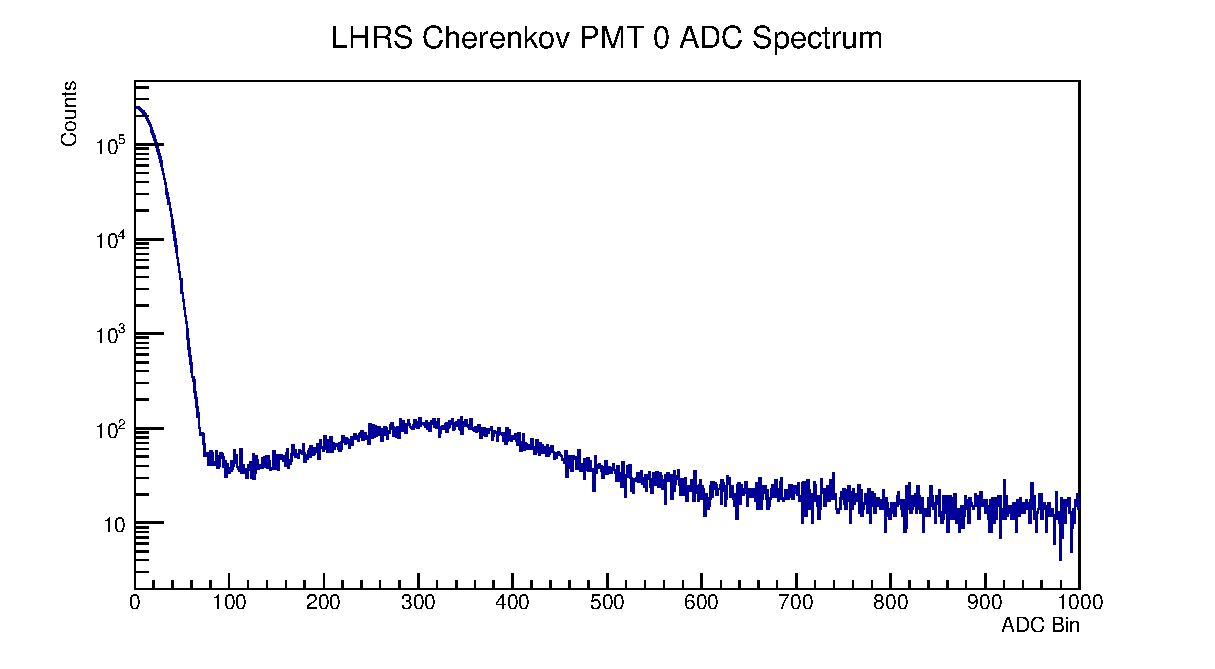
\includegraphics[width=0.7\textwidth]{./setup/fig/cer_pmt.eps}
	\caption{The Cherenkov PMTs are calibrated to have the single photo-electron peak centered at ADC bin 300. The peak at 0 is the ADC pedestal.}
	\label{fig:cer_pmt}
\end{center}
\end{figure}

\subsection{Leaded Glass Calorimeters}

Both arms have two leaded glass calorimeters, known as the preshower and shower detectors. When a particle enters a calorimeter, it interacts with the material by depositing energy. This energy is converted into an electromagnetic shower of photons which are detected by PMTs attached to the glass blocks. How much energy is deposited is dependent on the particle and its radiation length within the material. In the case of the HRSs, the calorimeters are thick enough that electrons will completely deposit all of their energy into the preshower and shower detectors. Each HRS has a slightly different configuration for the calorimeters.

In the LHRS, the preshower and shower blocks are all perpendicular to the path of the particle. Both layers have are comprised of 34 blocks at alternate in size between 15 cm x 15 cm x 30 cm and 15 cm x 15 cm x 35 cm.

In the RHRS, the preshower blocks are perpendicular to the path of the particle while the shower blocks are parallel to the path of the particle. The preshower layer is composed of 48 blocks that measure 10 cm x 10 cm x 35 cm. The shower layer is composed of 80 blocks that measure 15 cm x 15 cm x 35 cm.

The signal from the calorimeters is directly correlated to the energy of the particle that was detected. Typically for PID, a measure of $E/p$ is used, that is the ratio of energy to momentum of the detected particle. This allows for very efficient identification of particles because electrons will peak around 1 and larger particles will have a much lower ratio.

\begin{figure}
\begin{center}
	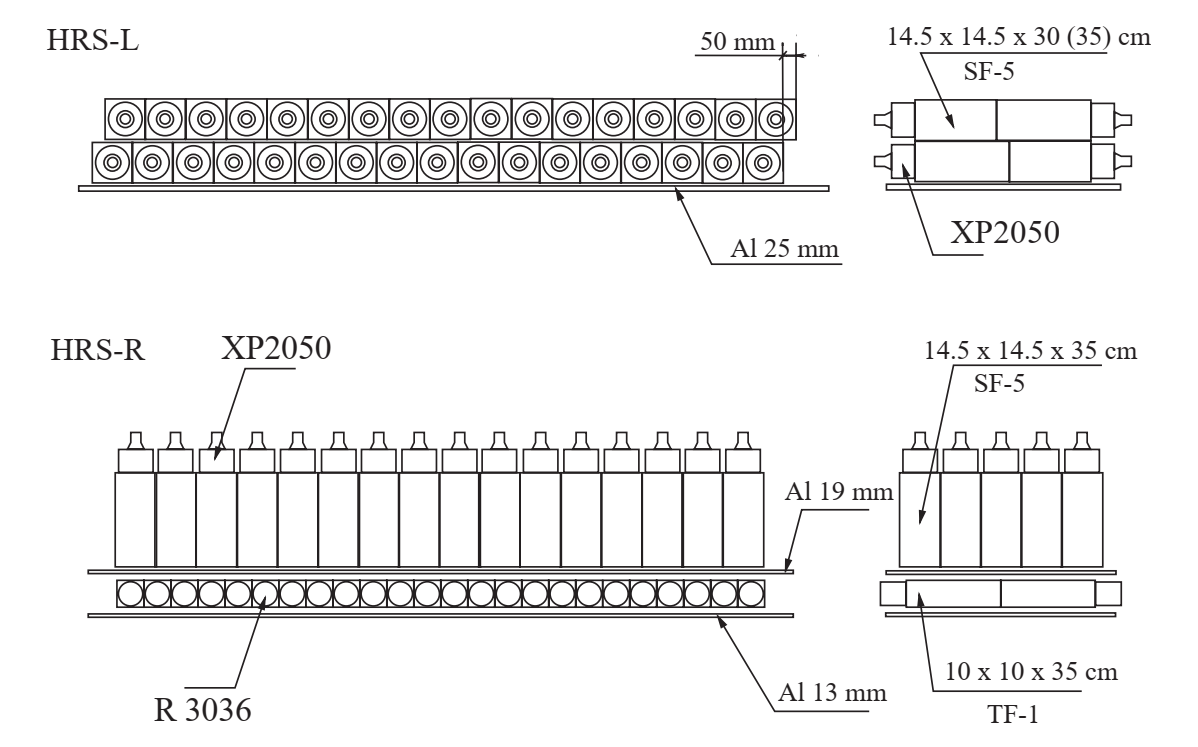
\includegraphics[width=0.8\textwidth]{./setup/fig/shower_layout.png}
	\caption{Layout of the shower blocks. Particles enter from the bottom of the page. Left is top-view. Right is side-view. \cite{HANIM}}
	\label{shower_layout}
\end{center}
\end{figure}

\subsection{Trigger}

The HRSs read in data from the described detectors through a combination of Fastbus ADCs and TDCs and VME Flash ADCs. A Trigger Supervisor (TS) unit is used to distribute a trigger signal to this hardware. This trigger signals the ADCs and TDCs to record this signal and send it to be written. This process is overseen by CEBAF Online Data Acquisition (CODA) software written at JLab. The CODA software communicates with the TS crate to signal when it is ready to receive data and that triggers should begin being processed.

In order to distribute a signal to the ADCs and TDCs, the TS unit must receive an outside trigger. A trigger is a logic signal that is generated to indicate that the data that would be recorded is potentially a ``good event''. This trigger is generated from the signals that are produced by the detectors in the HRSs.

To produce this trigger, signals received from the scintillators and cherenkov are processed by NIM electronics. First, the signals are scintillator PMT signals are ``discriminated''. Each of these signals are then passed through a discriminator which, provided the signals are large enough to exceed a set threshold signifying a real signal, converts the signal into a logic pulse. The length of these logic pulses is set to allow for timing the coincidence of these three detectors. The PMTs in each scintillator plane are then checked for coincidence, that is any signal received within a designated window of time is defined as being from the same event. In the setup for S0, both PMTs must have a signal for this process to consider there to have been an event. The S2 setup requires that any single paddle must have a signal from both PMTs in order to trigger. For the cherenkov, the PMT signals are summed and then discriminated. The logic pulses for each detector are then delayed to allow for timing of coincidence between detectors. The need for delaying the signals is due to the varying length of cables from the detectors to the processing hardware.

These logic signals are finally combined into four different triggers:
\begin{itemize}
	\item S0 \textbar\textbar{} S2
	\item S0 \&\& S2
	\item (S0 \textbar\textbar{} S2) \&\& Cherenkov
	\item (S0 \&\& S2) \&\& Cherenkov
\end{itemize}
Ultimately, the final three of these triggers were used in the experiment. These are referred to (sequentially) as Triggers 1-3. A schematic of formation of these signals can be seen in Figure \ref{fig:trig_schem}. In the formation of these triggers, the scintillators are used to set the timing for the TDCs. Particularly, S2 always sets the timing of the trigger since it has the highest timing resolution. In the case of the triggers where S0 and S2 are ``OR'd'', S0 will set the timing in the absence of an S2 signal.

\begin{figure}
\begin{center}
	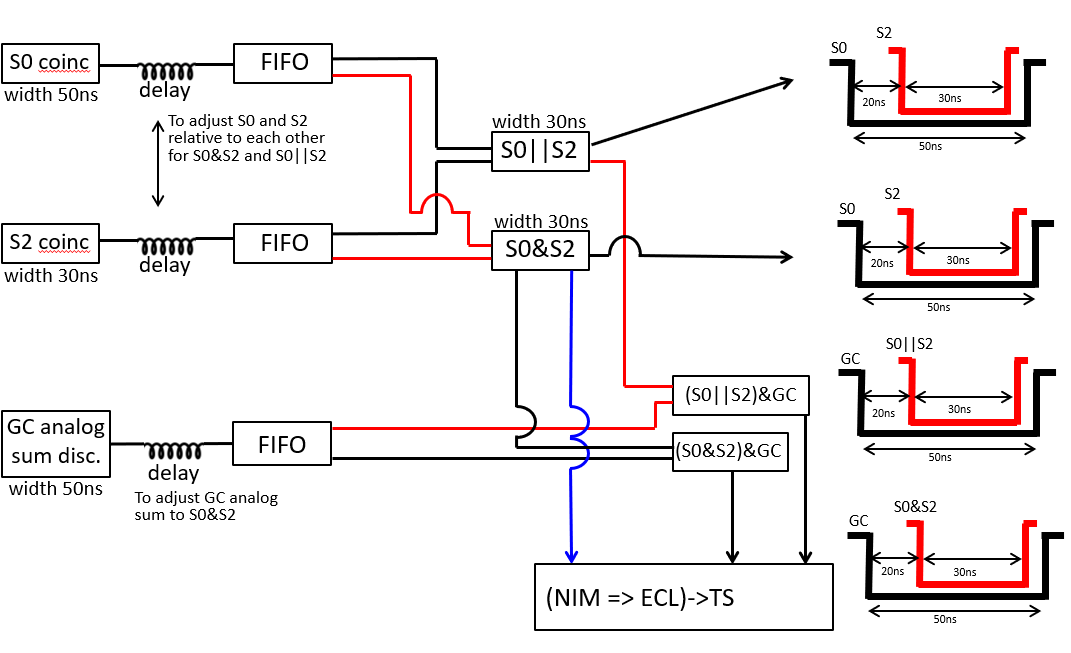
\includegraphics[width=\textwidth]{./setup/fig/trigger_diagram.png}
	\caption{A schematic diagram of the trigger setup for MARATHON. In this diagram ``disc.'' stands for discriminator. ``FIFO'' stands for ``Fan in fan out'', which is a unit that takes a signal and then outputs it to multiple channels. ``NIM=$>$ECL'' denotes the conversion from NIM to ECL logic standards which is necessary to interface with the Trigger Supervisor. The drawings on the right show the relative width of each signal to facilitate event timing.\cite{Rey}}
	\label{fig:trig_schem}
\end{center}
\end{figure}